\documentclass{standalone}
\usepackage{tikz}
\usepackage{ctex,siunitx}
\setCJKmainfont{Noto Serif CJK SC}
\usepackage{tkz-euclide}
\usepackage{amsmath}
\usetikzlibrary{patterns, calc}
\usetikzlibrary {decorations.pathmorphing, decorations.pathreplacing, decorations.shapes,}

\begin{document}
\small
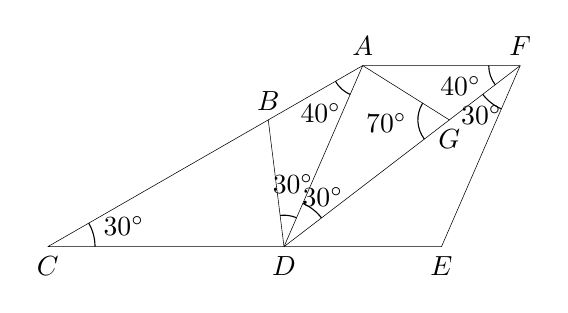
\begin{tikzpicture}[>=stealth,scale=1]
  \tkzSetUpPoint[fill=black]
  % \useasboundingbox(-1,-0.75)rectangle(3.7,1.4);
  \tkzDefPoints{0/0/C, 3/0/D, 5/0/E, 6/2.3/F}
  \tkzDefPointsBy[translation= from E to F](D){A}
  \tkzDrawPolygon(C,E,F,A)
  \tkzLabelPoints[below](C,D,E)
  \tkzLabelPoints[above](A,F)
  \tkzDrawSegments(A,D D,F)
  \tkzDefPointWith[linear, K=.7](C,A)\tkzGetPoint{B}
  \tkzDefPointWith[linear, K=.7](D,F)\tkzGetPoint{G}
  \tkzDrawSegments(B,D A,G)
  \tkzMarkAngles[mark=none, size=.6](D,C,B F,D,A D,F,E)
  \tkzMarkAngles[mark=none, size=.4](C,A,D A,G,D A,F,D A,D,B)
  \tkzLabelAngle[pos=1](D,C,B){$30^{\circ}$}
  \tkzLabelAngle[pos=.8](A,D,B){$30^{\circ}$}
  \tkzLabelAngle[pos=.8](F,D,A){$30^{\circ}$}
  \tkzLabelAngle[pos=.8](D,F,E){$30^{\circ}$}
  \tkzLabelAngle[pos=.8](C,A,D){$40^{\circ}$}
  \tkzLabelAngle[pos=.8](A,G,D){$70^{\circ}$}
  \tkzLabelAngle[pos=.8](A,F,D){$40^{\circ}$}
  \tkzLabelPoints[above](B)
  \tkzLabelPoints[below](G)
\end{tikzpicture}
\end{document}